\documentclass[20pt]{beamer}


\usepackage[size=a0,orientation=portrait,scale=1.4]{beamerposter}
\usepackage{changepage}

\usetheme{Madrid}

\graphicspath{{Images/}}


\renewcommand{\raggedright}{\leftskip=0pt \rightskip=0pt}
\let\olditemize\itemize
\renewcommand{\itemize}{\olditemize\addtolength{\itemsep}{0.4\baselineskip}}

\addtobeamertemplate{block begin}{}{\vspace{5mm} \begin{adjustwidth}{5mm}{5mm}}
\addtobeamertemplate{block end}{\end{adjustwidth}}{\vspace{5mm}}
\setbeamerfont{block title}{size={\centering\bfseries\fontsize{48}{60}\selectfont}}

\setbeamercolor{background canvas}{bg=green!75}

\definecolor{title-color}{RGB}{127 96 0}

\setbeamercolor{chcolor}{fg=white,bg=title-color}

\setbeamertemplate{headline}{%
\begin{beamercolorbox}[wd=\paperwidth]{chcolor}\vskip5mm

\begin{columns}

\begin{column}{0.15\linewidth}
\centering
		
\includegraphics[width=0.85\linewidth]{science}
\end{column}

\begin{column}{0.85\linewidth}
\centering\bfseries
{\fontsize{80}{96}\selectfont Black Hole Research }\\ [6mm]
{\fontsize{60}{72}\selectfont Dong Lee, Fahad }\\ [6mm]
{\fontsize{48}{60}\selectfont Department of Astrophysics, University of Berkeley,USA.}\\ [3mm]
{\fontsize{36}{42}\selectfont Email: author@gmail.com }\\ [3mm]
\end{column}

\end{columns}\vskip5mm
\end{beamercolorbox}

\color{red}\rule{\paperwidth}{20pt}
}

\setbeamercolor{chfootcolor}{fg=white,bg=black}

\setbeamercolor{block body}{bg=white}

\setbeamertemplate{footline}{
\begin{beamercolorbox}[wd=\paperwidth,center,ht=1.5em]{chfootcolor}
\small For any suggestions/queries: author@gmail.com
\end{beamercolorbox}
}

\begin{document}\vspace*{-2cm}
\begin{frame}[t]
\begin{columns}[t]

%============================Column 1===========================
\begin{column}{0.32\linewidth}

\begin{block}{Introduction}
A black hole is a region of space time where gravity is so strong that nothing no particles or even electromagnetic radiation such as light can escape from it. The theory of general relativity predicts that a sufficiently compact mass can deform space time to form a black hole. The boundary of the region from which no escape is possible is called the event horizon.

\begin{itemize}
 	\item Although the event horizon has an enormous effect on the fate and circumstances of an object crossing it, according to general relativity it has no locally detectable features.
 	
 	\item   In many ways, a black hole acts like an ideal black body, as it reflects no light. Moreover, quantum field theory in curved space time predicts that event horizons emit Hawking radiation, with the same spectrum as a black body of a temperature inversely proportional to its mass.
 	
 	\item  This temperature is on the order of billionths of a kelvin for black holes of stellar mass, making it essentially impossible to observe.
 	
\end{itemize}
 
\begin{figure}
		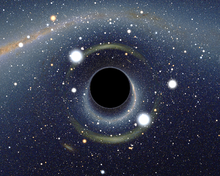
\includegraphics[width=\linewidth]{blackhole2.png}
		\caption{This is an example of black hole picture}		
\end{figure}

\end{block}

\begin{block}{Physical Properties}
The simplest static black holes have mass but neither electric charge nor angular momentum. 

\begin{itemize}

\item According to Birkhoff\'s theorem, it is the only vacuum solution that is spherically symmetric.

\item  This means there is no observable difference at a distance between the gravitational field of such a black hole and that of any other spherical object of the same mass.

\item  The popular notion of a black hole sucking in everything in its surroundings is therefore correct only near a black hole\'s horizon; far away, the external gravitational field is identical to that of any other body of the same mass.

\end{itemize}
 
\begin{figure}
	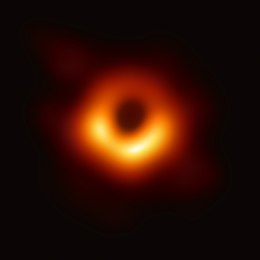
\includegraphics[scale=2.5]{blackhole.jpg}
 	\caption{ This is the example of black hole picture }

\end{figure}[

\end{block}

\end{column}

%===========================Column 2=============================

\begin{column}{0.32\linewidth}

\begin{block}{General relativity}
In 1915, Albert Einstein developed his theory of general relativity, having earlier shown that gravity does influence light's motion. 

\begin{itemize}

\item  A few months after Schwarzschild, Johannes Droste, a student of Hendrik Lorentz, independently gave the same solution for the point mass and wrote more extensively about its properties.

\item  This solution had a peculiar behaviour at what is now called the Schwarzschild radius, where it became singular, meaning that some of the terms in the Einstein equations became infinite.

\item The nature of this surface was not quite understood at the time. In 1924, Arthur Eddington showed that the singularity disappeared after a change of coordinates (see Eddington–Finkelstein coordinates), although it took until 1933 for Georges Lemaître to realize that this meant the singularity at the Schwarzschild radius was a non-physical coordinate singularity.

\end{itemize}

\end{block}


\begin{block}{Accretion of matter}
	Due to conservation of angular momentum, gas falling into the gravitational well created by a massive object will typically form a disk-like structure around the object.
\begin{itemize}
  
  \item Artists impressions such as the accompanying representation of a black hole with corona commonly depict the black hole as if it were a flat-space body hiding the part of the disk just behind it, but in reality gravitational lensing would greatly distort the image of the accretion disk.

  \item NASA simulated view from outside the horizon of a Schwarzschild black hole lit by a thin accretion disk.
	
 \item Within such a disk, friction would cause angular momentum to be transported outward, allowing matter to fall farther inward, thus releasing potential energy and increasing the temperature of the gas.

\end{itemize}
 



\end{block}

\begin{block}{X-ray binaries}
X-ray binaries are binary star systems that emit a majority of their radiation in the X-ray part of the spectrum. These X-ray emissions are generally thought to result when one of the stars (compact object) accretes matter from another (regular) star.

\begin{itemize}

	\item The presence of an ordinary star in such a system provides an opportunity for studying the central object and to determine if it might be a black hole.

	\item If such a system emits signals that can be directly traced back to the compact object, it cannot be a black hole. The absence of such a signal does, however, not exclude the possibility that the compact object is a neutron star.
	
	\item  By studying the companion star it is often possible to obtain the orbital parameters of the system and to obtain an estimate for the mass of the compact object.
	
	\item If this is much larger than the Tolman–Oppenheimer–Volkoff limit (the maximum mass a star can have without collapsing) then the object cannot be a neutron star and is generally expected to be a black hole.
	
\end{itemize}
 
\end{block}

\end{column}

%==========================Column 3==============================

\begin{column}{0.32\linewidth}

\begin{block}{Galactic nuclei}
	Astronomers use the term active galaxy to describe galaxies with unusual characteristics, such as unusual spectral line emission and very strong radio emission. 
	
\begin{itemize}

\item Theoretical and observational studies have shown that the activity in these active galactic nuclei (AGN) may be explained by the presence of super massive black holes, which can be millions of times more massive than stellar ones.

\item The models of these AGN consist of a central black hole that may be millions or billions of times more massive than the Sun a disk of gas and dust called an accretion disk; and two jets perpendicular to the accretion disk.

\end{itemize}	
	 
\end{block}

\begin{block}{Micro lensing}
Another way the black hole nature of an object may be tested in the future is through observation of effects caused by a strong gravitational field in their vicinity. 

\begin{itemize}

\item One such effect is gravitational lensing: The deformation of space time around a massive object causes light rays to be deflected much as light passing through an optic lens.

\item Observations have been made of weak gravitational lensing, in which light rays are deflected by only a few arc seconds.

\item However, it has never been directly observed for a black hole. One possibility for observing gravitational lensing by a black hole would be to observe stars in orbit around the black hole.

\item  There are several candidates for such an observation in orbit around Sagittarius A*.

\end{itemize}

\end{block}

\begin{block}{Entropy and thermodynamics}
In 1971, Hawking showed under general conditions that the total area of the event horizons of any collection of classical black holes can never decrease, even if they collide and merge.

\begin{itemize}

\item This result, now known as the second law of black hole mechanics, is remarkably similar to the second law of thermodynamics, which states that the total entropy of an isolated system can never decrease.

\item As with classical objects at absolute zero temperature, it was assumed that black holes had zero entropy.

\item If this were the case, the second law of thermodynamics would be violated by entropy-laden matter entering a black hole, resulting in a decrease of the total entropy of the universe.

\item Therefore, Bekenstein proposed that a black hole should have an entropy, and that it should be proportional to its horizon area.

\end{itemize}
    
\end{block}

\begin{block}{Information loss paradox}
Because a black hole has only a few internal parameters, most of the information about the matter that went into forming the black hole is lost. 
\begin{enumerate}

\item As long as black holes were thought to persist forever this information loss is not that problematic, as the information can be thought of as existing inside the black hole, inaccessible from the outside, but represented on the event horizon in accordance with the holographic principle.

\item However, black holes slowly evaporate by emitting Hawking radiation. This radiation does not appear to carry any additional information about the matter that formed the black hole, meaning that this information appears to be gone forever.

\end{enumerate}

\end{block}

\end{column}



\end{columns}
\end{frame}
\end{document}